\documentclass[a4paper]{article}
\usepackage[spanish]{babel}
\usepackage[utf8]{inputenc}
\usepackage{charter}   % tipografia
\usepackage{graphicx}
\usepackage{wrapfig}
\usepackage[dvipsnames]{xcolor}
\usepackage{textcomp}
%\usepackage{makeidx}

%\usepackage{float}
%\usepackage{amsmath, amsthm, amssymb}
%\usepackage{amsfonts}
%\usepackage{sectsty}
%\usepackage{charter}
%\usepackage{wrapfig}
%\usepackage{listings}
%\lstset{language=C}

\usepackage{color} % para snipets de codigo coloreados
\usepackage{fancybox}  % para el sbox de los snipets de codigo

\definecolor{litegrey}{gray}{0.94}

% \newenvironment{sidebar}{%
% 	\begin{Sbox}\begin{minipage}{.85\textwidth}}%
% 	{\end{minipage}\end{Sbox}%
% 		\begin{center}\setlength{\fboxsep}{6pt}%
% 		\shadowbox{\TheSbox}\end{center}}
% \newenvironment{warning}{%
% 	\begin{Sbox}\begin{minipage}{.85\textwidth}\sffamily\lite\small\RaggedRight}%
% 	{\end{minipage}\end{Sbox}%
% 		\begin{center}\setlength{\fboxsep}{6pt}%
% 		\colorbox{litegrey}{\TheSbox}\end{center}}

\newenvironment{codesnippet}{%
	\begin{Sbox}\begin{minipage}{\textwidth}\sffamily\small}%
	{\end{minipage}\end{Sbox}%
		\begin{center}%
		\colorbox{litegrey}{\TheSbox}\end{center}}



\usepackage{fancyhdr}
\pagestyle{fancy}

%\renewcommand{\chaptermark}[1]{\markboth{#1}{}}
\renewcommand{\sectionmark}[1]{\markright{\thesection\ - #1}}

\fancyhf{}

%\fancyhead[LO]{Sección \rightmark} % \thesection\ 
\fancyfoot[LO]{\small{Ciruelos Rodríguez Gonzalo, Maddonni Axel, Thibeault Gabriel}}
\fancyfoot[RO]{\thepage}
\renewcommand{\headrulewidth}{0.5pt}
\renewcommand{\footrulewidth}{0.5pt}
\setlength{\hoffset}{-0.8in}
\setlength{\textwidth}{16cm}
%\setlength{\hoffset}{-1.1cm}
%\setlength{\textwidth}{16cm}
\setlength{\headsep}{0.5cm}
\setlength{\textheight}{25cm}
\setlength{\voffset}{-0.7in}
\setlength{\headwidth}{\textwidth}
\setlength{\headheight}{13.1pt}

\renewcommand{\baselinestretch}{1.1}  % line spacing


% \setcounter{secnumdepth}{2}
\usepackage{underscore}
\usepackage{caratula}
\usepackage{url}
\usepackage{float}


% ******************************************************** %
%              TEMPLATE DE INFORME ORGA2 v0.1              %
% ******************************************************** %
% ******************************************************** %
%                                                          %
% ALGUNOS PAQUETES REQUERIDOS (EN UBUNTU):                 %
% ========================================
%                                                          %
% texlive-latex-base                                       %
% texlive-latex-recommended                                %
% texlive-fonts-recommended                                %
% texlive-latex-extra?                                     %
% texlive-lang-spanish (en ubuntu 13.10)                   %
% ******************************************************** %
\usepackage{listings}


\renewcommand{\lstlistingname}{Codigo}
% Lenguajes soportados: ftp://ftp.tex.ac.uk/tex-archive/macros/latex/contrib/listings/listings.pdf
\lstloadlanguages{[ANSI]C} 
% FIXME: Me robe lo de abajo de otro ejemplo, estaba basado en Perl, ver si hay que cambiar algo
%\lstset{language=[x86masm]Assembler,
\lstset{language=[ANSI]C,
        frame=single,
        breaklines=true, 			% Saltar de linea si supero el maximo
        basicstyle=\small\ttfamily,
        keywordstyle=[1]\color{Blue}\bf,	% Color de las funciones de assembler
        keywordstyle=[2]\color{Purple},		% Color de parámetros especiales (registros, etc)
        identifierstyle=,                               
        commentstyle=\usefont{T1}{pcr}{m}{sl}\color{DarkGreen}\small,
        stringstyle=\color{Purple},     	% Strings purpuras
        showstringspaces=false,
        tabsize=4,
        %
        % Instrucciones no incluidas en el paquete Assembler
        morekeywords={global, define, section, .rodata, .text, jl, movd, movdqu, mulss, subss, addss, cmpss, pand, cvtss2si, cvttss2si, cvtsi2ss},
        %
        % Registros y esas otras cosas especiales que no son instrucciones
        morekeywords=[2]{rax,rdx,rcx,rbx,rsi,rdi,rsp,rbp,r8,r9,r10,r11,r12,r13,r14,r15,xmm0,xmm1,xmm2,xmm3,xmm4,xmm5,xmm6,xmm7
        		xmm8,xmm9,xmm10,xmm11,xmm12,xmm13,xmm14,xmm15,r8b, r9b, r10b, r11b, r8d, r9d, r10d, r11d},
       	%
        morecomment=[l][\color{Blue}]{...}, % Line continuation (...) like blue comment
        numbers=left, % Numeros de linea en la izquiera
        firstnumber=0, % Se arranca en la linea 1
        numberstyle=\tiny\color{Blue}, % Numeros de linea en azul y chicos
        stepnumber=0 % Los numerros de linea se muestran cada 5
}

\begin{document}

\thispagestyle{empty}
\materia{Organización del Computador II}
\submateria{Primer Cuatrimestre de 2015}
\titulo{Trabajo Práctico 3}
\subtitulo{System Programming - Tierra Pirata}
\grupo{Grupo Diablo II / PC}
\integrante{Ciruelos Rodríguez, Gonzalo}{063/14}{gonzalo.ciruelos@gmail.com} % obligatorio 
\integrante{Maddonni, Axel}{200/14}{axel.maddonni@gmail.com} % obligatorio 
\integrante{Thibeault, Gabriel}{}{} % obligatorio 

\maketitle
\newpage

\thispagestyle{empty}
\vfill

\thispagestyle{empty}
\vspace{3cm}
\tableofcontents
\newpage

%\normalsize
\newpage

\section{Introducción}

Los sistemas operativos son el software que se ocupa de manejar y administrar los recursos del hardware y proveer servicios a los programas. Sin sistemas operativos sólidos, realizar la mayoría de las tareas que realizamos hoy con las computadoras serían imposibles.

En este trabajo nos proponemos aprender y entender como funcionan los mecanismos básicos que implementa un sistema operativo para manejar la memoria, manejar interrupciones, alternar tareas, etc.

A lo largo de la historia existieron muchos paradigmas de sistemas operativos, en general atados a las capacidades tecnológicas de la época. 
En este TP nos proponemos hacer un sistema operativo que trabaja en modo protegido de 32 bits, con paginación y multitarea.
Teniendo esas características, nuestro sistema operativo \emph{de juguete} es más avanzado en varios aspectos que el DOS original de Microsoft (que trabajaba en modo real y era monotarea), por lo que sentimos que va a ser un interesante desafío.
\\

Para testear nuestro kernel durante el proceso de desarrollo utilizamos el software \texttt{Bochs}, un proyecto de código abierto, que permite emular una IBM PC tanto de 32 bits, como de 64 bits. Tambien permite emular dispositivos y un BIOS, por lo cual es ideal para el desarrollo de sistemas operativos.



\newpage

\section{Desarrollo} 
	\par La explicación de la implementación del sistema está dividida según los ejercicios planteados por el enunciado. Al final, se encuentra un apéndice con una breve explicación sobre las estructuras del juego creadas para almacenar la información del juego.
\par A continuación, cómo está dividido el desarrollo y qué se encuentra en cada ejercicio:
\begin{itemize}
\item Ejercicio 1: Inicialización de la GDT, Pasaje a Modo Protegido e Inicialización de la Pantalla. 
\item Ejercicio 2: Inicialización de la IDT.
\item Ejercicio 3: Inicialización de directorio y tablas de páginas de kernel y Activación de Paginación. 
\item Ejercicio 4: Inicialización de la MMU, Mapeo y Desmapeo de Páginas, Inicialización de directorios y tablas para tareas Pirata.
\item Ejercicio 5: Interrupción de Reloj, Interrupción de Teclado e Interrupción de syscalls 0x46.
\item Ejercicio 6: Inicialización de las TSS, Rutinas de atención de servicios para MOVER, CAVAR y calcular POSICION de piratas, ejecución de tareas.
\item Ejercicio 7: Inicialización del Scheduler y sus funciones, Modo Debugger.
\item Apéndice: Descripción de los struct_Pirata y struct_Jugador para almacenar información sobre el juego, y funciones auxiliares.
\end{itemize}

\newpage

\subsection{Ejercicio 1}
	\subsubsection*{Inicialización de la GDT}

Inicializamos la Tabla de Descriptores Globales con entradas para segmentos de código de nivel 0 y 3, otras para segmentos de datos de nivel 0 y 3, una para un segmento que describe el área de la pantalla de video, y la entrada correspondiente al segmento donde se guardará la tss de la tarea inicial. (Las entradas de gdt para las tss de las demás tareas son completadas al inicializarlas, como se explica en la sección correspondiente al Ejercicio 6).

\par Se utiliza desde el índice 8 por restricciones del trabajo práctico.
Los segmentos de datos y códigos están organizados de tal forma que se superpongan direccionando los primeros 500MB de memoria (Sistema FLAT), utilizando bloques de 4K al setear el bit de granularidad en 1.
\par Los demás atributos fueron seteados de la siguiente manera:
\par \textbf{\emph{Base y Límite: } }Como mencionamos anteriormente, los segmentos de código y datos están superpuestos. Comienzan en la dirección base 0x00000000, y el valor del límite 0x1F3FF corresponde la cantidad de bloques-1. Es decir, para cubrir 500MB se necesitan 128.000 bloques de 4K. El offset del último bloque es 127.999 (0x1F3FF en hexa).
Con respecto al segmento de video, éste ocupa en memoria desde la posición 0xB8000 hasta la 0xC0000, es decir 32K de memoria, cuyo máximo offset o límite es el correspondiente al último byte (7999 = 0x7FFF).
Para las tss, el límite es 0x68, pues miden 104 bytes cada una. Como base de la tarea inicial, seteamos la dirección 0x0000. ???????
\par \emph{\textbf{Tipo: }} El tipo para los segmentos de código es 0x0A (executable, readable), mientras que para los de datos y video es 0x02 (readable, writable).
\par \emph{\textbf{Sistema: }} El bit de system está seteado en 1 salvo en los segmentos correspondientes a las tss de las tareas, donde está activo bajo en 0 pues son potestad exclusiva del sistema operativo.
\par \emph{\textbf{DPL: }} Los segmentos de datos y código de nivel 0 tienen DPL en 0x00, al igual que los segmentos de sistema y el de video, mientras que los de código y datos nivel 3 tienen DPL en 0x03.
\par \emph{\textbf{Granularidad: }} El bit de G está activo sólo en los segmentos de datos y código ya que es necesario bloques de 4K para abarcar los 500MB.
\par \emph{\textbf{P, L, D/B, AVL: } }Seteados en 1, 0, 1 y 0 respectivamente para todas las entradas.
\newline

\subsubsection*{Pasaje a Modo Protegido}

\par Para pasar a modo protegido, completamos y cargamos la GDT usando la instrucción lgdt, que toma el descriptor de la GDT con el tamaño y la dirección de la misma, habilitamos A20 para habilitar el acceso a direcciones superiores a los 2$^{20}$ bits, seteamos el bit de PE del registro CR0, y saltamos a 0x40:modoprotegido donde el 0x40 corresponde al Indice del segmento de código de nivel 0 (índice 8 en la gdt), corrido 3 ceros (estos ceros son los del TI y RPL).

\begin{lstlisting} [caption={Pasaje a modo protegido},label=modoproteg]
    ; Habilitar A20
    call habilitar_A20  
   
    ; Cargar la GDT
	lgdt [GDT_DESC]      ; cargo la estructura que esta en gdt.c

    ; Setear el bit PE del registro CR0
    mov eax, cr0
	or eax, 1
	mov cr0, eax

    ; Saltar a modo protegido
	jmp 0x40:modoprotegido
\end{lstlisting}


\par Una vez trabajando en modo protegido, procedemos a establecer los selectores de segmentos de datos de nivel 0 (indice 9 en la gdt, corrido tres ceros correspondientes a los bits de TI y RPL), y el selector de segmento de video en fs (indice 12 en la gdt). Luego establecemos la base de la pila en la dirección 0x27000.


\begin{lstlisting} [caption={Pasaje a modo protegido},label=modoproteg2]
    modoprotegido:
    ;Establecer selectores de segmentos
    xor eax, eax
	mov ax,  1001000b
	mov ds, ax
	mov es, ax
	mov gs, ax
	mov ss, ax
    	mov ax, 1100000b
    mov fs, ax

    ; Establecer la base de la pila
	mov ebp, 0x27000
	mov esp, 0x27000
\end{lstlisting}

\subsubsection*{Inicialización de la Pantalla}

\par Para inicializar la pantalla llamamos a la función de screen.h \texttt{screen_inicializar}, que se encarga de pintar la pantalla con el mapa, las barras para los jugadores, e inicializar los slots vacios y puntos en 0 de cada jugador, utilizando las funciones \texttt{screen_pintar_rect} para pintar un rectangulo de color, \texttt{print_dec} para imprimir los puntos, y \texttt{screen_pintar} para imprimir caracteres.

\begin{figure}[ht!]
\centering
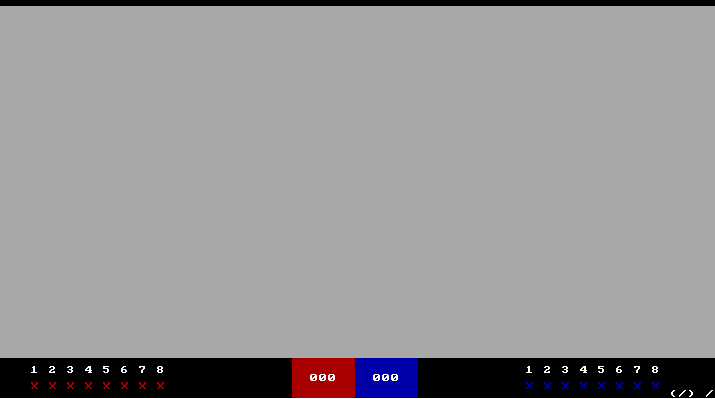
\includegraphics[width=120mm]{imagenes/pantalla.png}
\caption{Pantalla Inicial.}
\end{figure}

\newpage

\subsection{Ejercicio 2}
	\subsubsection*{Inicialización de la IDT}

\par Para inicializar la IDT se llama a una funci\'on en lenguaje C, "void idt\_inicializar(void)". La IDT se representa mediante un arrelgo (de tama\~no 255) de "idt\_entry"
(esta estructura fue definida como lo muestra el extracto de C\'odigo \ref{idtEntry}, seg\'un las especificaciones dadas en el manual de Intel). Esta funci\'on utiliza un macro
(que se encuentra en el extracto de C\'odigo \ref{macro}) para inicializar cada una de las entradas necesarias de la IDT. 
\par El macro define el offset como los 16 bits menos y m\'as significativos (ya que \'este se encuentra separado en dos campos de 16 bits cada uno) de la direcci\'on de la tarea de atenci\'on
de la interrupci\'on correspondiente. El selector de segmento lo define como 0x0040, que es 0x8 (el indice del segmento de codigo de nivel de privilegio 0 en la GDT) shifteado 3 bits a la izquierda.
Los atributos los define como 0x8e00, que representan un segmento presente (P = 1), un nivel de privilegio de 0 (DPL = 00), un tama\~no de Gate de 32 bits (bits 8 a 12 de la Interrupt Gate = 0b01110),
y los 7 bits restantes en 0. 
\par Cabe destacar la entrada de la IDT correspondiente a la interrupci\'on 0x46 (correspondiente a las \textit{syscalls}), que se inicializa de la forma detallada en el extracto de c\'odigo \ref{0x46}
. La \'unica diferencia entre esta entrada y la definida por el macro previamente mencionado son los atributos, puntualmente el DPL (3 en esta entrada y 0 en las otras); esta diferencia se debe a que la \textit{syscall} debe poder ser llamada por las tareas, mientras que las otras interrupciones deben estar reservadas al nivel m\'as privilegiado.
\par La rutina de atenci\'on de cada interrupci\'on se genera a partir de un macro (que se encuentra en el extracto de C\'odigo \ref{macroISR}) que imprime el c\'odigo de error correspondiente
a pantalla y luego queda en un loop infinito (esta rutina es un placeholder, que luego ser\'a reemplazada por una que mate a la tarea que causa la interrupci\'on y llame a la idle).
\par La IDT ya inicializada se puede acceder tras ejecutar la instrucci\'on $lidt [IDT\_DESC]$. El descriptor de la IDT, "IDT\_DESC" es una estructura (definida como se ve en el extracto de
c\'odigo \ref{idtDesc}) que contiene el tama\~no de la IDT y su direcci\'on en memoria.

\begin{lstlisting} [caption={Estructura de idt\_entry},label=idtEntry]
typedef struct str_idt_entry_fld {
    unsigned short offset_0_15;
    unsigned short segsel;
    unsigned short attr;
    unsigned short offset_16_31;
} __attribute__((__packed__, aligned (8))) idt_entry;

\end{lstlisting}


\begin{lstlisting} [caption={Codigo del macro utilizado para inicializar la IDT},label=macro]
#define IDT_ENTRY(numero)                                                                                        
    idt[numero].offset_0_15 = (unsigned short) ((unsigned int)(&_isr ## numero) & (unsigned int) 0xFFFF);        
    idt[numero].segsel = (unsigned short) 0x0040;                                                                
    idt[numero].attr = (unsigned short) 0x8e00;                                                                  
    idt[numero].offset_16_31 = (unsigned short) ((unsigned int)(&_isr ## numero) >> 16 & (unsigned int) 0xFFFF);
\end{lstlisting}

\begin{lstlisting} [caption={Codigo del macro utilizado para la rutina de atencion de interrupciones},label=macroISR]
_isr%1:
    mov eax, %1
    push dword 0x0f0f 
    push dword 0
    push dword 0
    push MENSAJE_ERROR_%1
    call print
    
    jmp \$
\end{lstlisting}

\begin{lstlisting} [caption={Estructura de IDT\_Desc}],label=idtDesc] 
typedef struct str_idt_descriptor {
    unsigned short  idt_length;
    unsigned int    idt_addr;
} __attribute__((__packed__)) idt_descriptor;
\end{lstlisting}

\begin{lstlisting} [caption={Codigo de la entrada de IDT de int 0x46},label=0x46]
#define IDT_ENTRY(numero)                                                                                        
    idt[numero].offset_0_15 = (unsigned short) ((unsigned int)(&_isr ## numero) & (unsigned int) 0xFFFF);        
    idt[numero].segsel = (unsigned short) 0x0040;                                                                
    idt[numero].attr = (unsigned short) 0xee00;                                                                  
    idt[numero].offset_16_31 = (unsigned short) ((unsigned int)(&_isr ## numero) >> 16 & (unsigned int) 0xFFFF);
\end{lstlisting}




\newpage

\subsection{Ejercicio 3}
	\subsubsection*{Inicialización de de directorio y tablas de kernel}

\par Para inicializar el directorio del kernel, lo que hacemos es, en la primera posición declarar la tabla de kernel (que será identity mapping), y luego ponemos todo el resto de directorio en 0 (bit de presente en 0, que indica que esas entradas no direccionan nada).

\par Luego inicializamos la tabla de kernel, que está en identity mapping, como dijimos anteriormente. Eso es bastante fácil, ya que podemos usar la misma variable para iterar y para decir la dirección física a la que direccionará una dirección virtual.

\subsubsection*{Activación de Paginación}

\par Para habilitar paginación, una vez inicializado correctamente el mmu, activamos el bit de PE del registro cr0:
\begin{lstlisting} [caption={Paginación en kernel.asm}],label=paginacion] 
    mov eax, cr0
    or eax, 0x80000000
    mov cr0, eax
\end{lstlisting}
    
\subsubsection*{Imprimir en pantalla}

\par Para pintar la pantalla usamos las funciones que nos permiten pintar rectángulos, que no necesitan explicación dado que son muy simples. (más de screen.h en funciones auxiliares)

\newpage

\subsection{Ejercicio 4}
	\subsubsection*{Inicialización de la MMU}

\par Para administrar la memoria en el área libre contamos con un contador de páginas inicializado en la dirección 0x00100000. A medida que el sistema necesita una página,  éste contador se incrementa en 4K, como muestra la siguiente implementación:

\begin{lstlisting} [caption={Contador de Páginas Libres}],label=mmucontador] 
void * siguiente_libre;

void inicializar_mmu()
{
  siguiente_libre = (void *) PAGE_COUNTER_INIT;
}

void * dar_siguiente()
{
    uint i;
    for(i = 0; i<1024; i++) ((pde *) siguiente_libre)[i].present = 0;
    siguiente_libre += 0x1000;
    return siguiente_libre - 0x1000;
}
\end{lstlisting}

\par Al crear una página, recorremos todas entradas de la tabla seteando el bit de presente en 0 (sea ésta un directorio o tabla de páginas). Para simplificar la manipulación en el código de las pde y pte creamos dos estructuras en C correspondientes a las ya mencionadas: 

\begin{lstlisting} [caption={struct Page Directory Entry}],label=mmupde] 
typedef struct pde_t {
    unsigned char present:1;
    unsigned char read_write:1;
    unsigned char user_supervisor:1;
    unsigned char page_level_write_through:1;
    unsigned char page_level_cache_disable:1;
    unsigned char accessed:1;
    unsigned char reserved:1;
    unsigned char page_size:1;
    unsigned char global:1;
    unsigned char available_9_11:3;
    unsigned int  base_address:20;
} __attribute__((__packed__, aligned (4))) pde;
\end{lstlisting}

\begin{lstlisting} [caption={struct Page Table Entry}],label=mmupte] 
typedef struct pte_t {
    unsigned char present:1;
    unsigned char read_write:1;
    unsigned char user_supervisor:1;
    unsigned char page_level_write_through:1;
    unsigned char page_level_cache_disable:1;
    unsigned char accessed:1;
    unsigned char dirty:1;
    unsigned char page_table_attribute_index:1;
    unsigned char global:1;
    unsigned char available_9_11:3;
    unsigned int  base_address:20;
} __attribute__((__packed__, aligned (4))) pte;
\end{lstlisting}

\subsubsection*{Mapeo y Desmapeo de Páginas}

\par \texttt{mmu_mapear_pagina} toma una dirección lineal virtual, una dirección física, un directorio de tablas de página, y dos chars para indicar read/write y user/supervisor. La rutina realiza lo siguiente:
\begin{itemize}
\item (1) Se fija si el pde indicado por los 10 bits más significativos de la dirección lineal está presente en el directorio de páginas pasado por parámetro.
\item  (2) Si no está presente, crea una tabla de páginas con los atributos pasados por parámetro, y modifica la pde correspondiente en el directorio, para que apunte a ella.
\item (3) Luego, modifica la pte indicada por los siguientes 10 bits más significativos, como indica la figura, de la tabla creada (o modifica la ya existente en caso en que estaba en presente), cambiando el base address por la dirección física pasada por parámetro, corrida 12 bits correspondientes al offset, ya que las páginas están alineadas a 4k. El offset para buscar un dato dentro de ellas está en los 12 bits menos significativos de la dirección lineal.
\end{itemize}
\begin{figure}[ht!]
\centering
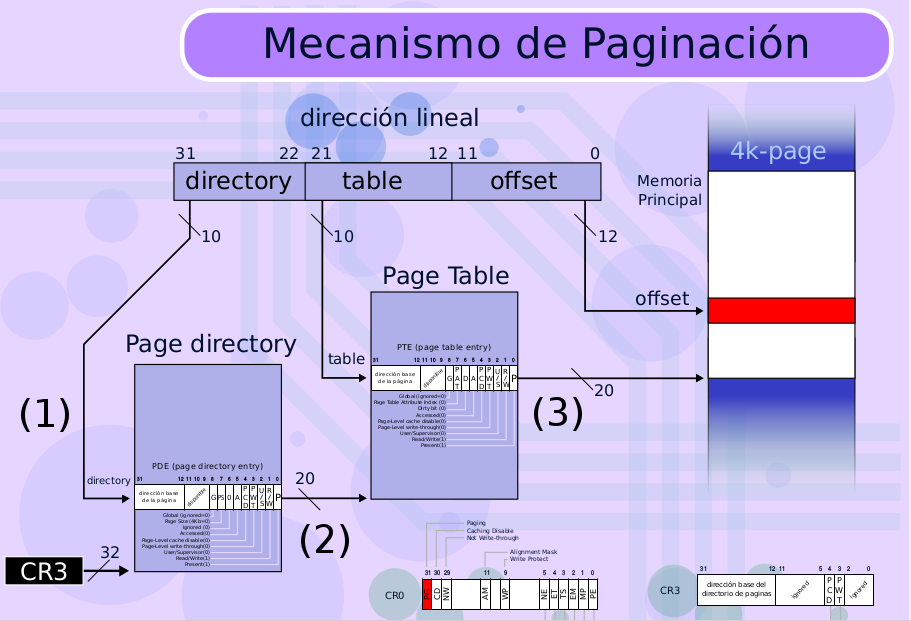
\includegraphics[width=100mm]{imagenes/paginacion.png}
\caption{Mapeo de Páginas}
\end{figure}

\par Análogamente, \texttt{mmu_unmapear_pagina} toma una dirección lineal y un directorio de tablas de página, y lo que hace es buscar primero la pde correspondiente en el directorio, indicado por los 10 bits más significativos, luego en dicha tabla busca la pte indicada por los siguientes 10 bits de la dirección lineal, y coloca el bit de presente de dicha entrada en 0.

\par Por la construcción del kernel, las direcciones de los mapas de memoria están mapeadas con indentity mapping. Como en estas funciones se modifica el directorio y/o tablas de páginas, al final se llama a \texttt{tlbflush() }para que se invalide la cache de traducción de direcciones. 

\subsubsection*{Inicialización de directorios y tablas para Tareas Pirata}

\par La rutina \texttt{mmu_inicializar_dir_pirata} se encarga de inicializar un directorio de páginas y tablas de páginas para una tarea, respetando la organización de la memoria establecida por el enunciado como muestra la siguiente figura:

\begin{figure}[ht!]
\centering
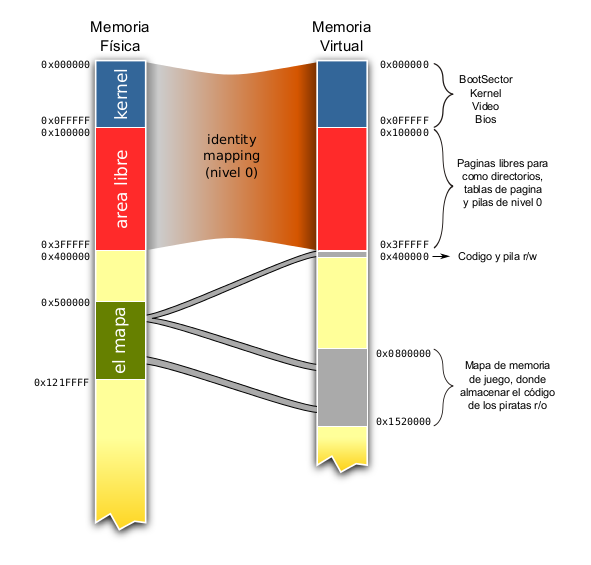
\includegraphics[width=100mm]{imagenes/memoriatarea.png}
\caption{Mapa de memoria de la Tarea.}
\end{figure}

\par Para lograr esto, la función toma como parámetros el jugador, el pirata y los parámetros que escribirá en la pila y luego utilizará la tarea. La rutina realiza lo siguiente:
\begin{itemize}
\item Obtenemos una página nueva usando la función previamente mencionada \texttt{dar_siguiente} para el directorio, y otra para la tabla de páginas del kernel. La tabla del kernel la inicializamos con la función \texttt{mmu_inicializar_tabla_kernel_para_pirata}, que básicamente hace una copia de la original, mapeando con identiy mapping las direcciones 0x00000000 a 0x003FFFFF como fue explicado en el ejercicio 3.

\item La primera entrada del directorio de páginas de la tarea se completa con la dirección base de la tabla de kernel inicializada en el item anterior, con los bits de read/write en 0, presente en 1, user/supervisor en 0 y reserved en 0, ya que sólo será accedido por las interrupciones del sistema de nivel 0, y sólo será de lectura.

\item Mapeamos las páginas de las posiciones exploradas del jugador entre las posiciones 0x0800000 y 0x1520000 como indica la figura. Para ello, recorremos la matriz de posiciones del mapa, y para aquellas que hayan sido exploradas por el jugador, calculamos su indice de página y mapeamos a la dirección correspondiente usando la función \texttt{mmu_mapear_pagina}.
\begin{lstlisting} [caption={Mapeo de páginas de posiciones exploradas.}],label=mmudirpirata1] 
 for(i = 0; i<MAPA_ALTO; i++){
     for(j = 0; j<MAPA_ANCHO; j++){
     	if(jugador->posiciones_exploradas[i][j]){
                uint ind = (i*MAPA_ANCHO+j) * 0x1000;
                mmu_mapear_pagina(0x800000+ind, resultado, 0x500000+ind, 0, 1);
            }
        }
    }
\end{lstlisting}

\item Mapeamos usando nuevamente \texttt{mmu_mapear_pagina} en la dirección virtual 0x400000 del directorio de la tarea, la dirección física correspondiente a la posición inicial del pirata, es decir, el puerto de donde sale. Dicha dirección se calcula usando la función auxiliar dada \texttt{game_xy2lineal}, que dada la posición inicial del pirata (la tenemos guardada en un array en cada struct del jugador), devuelve el índice de la página de memoria física a partir de la dirección 0x500000 correspondiente a esa posición del mapa.
\begin{lstlisting} [caption={Mapeo de la página correspondiente a la posición inicial.}],label=mmudirpirata2] 
mmu_mapear_pagina(0x400000, resultado, game_xy2lineal(p[0],p[1])*0x1000+0x500000, 1, 1);
\end{lstlisting}

\item Por último, queda copiar el código de la tarea correspondiente a la página de la posición inicial del pirata (mapeada en el paso anterior en el directorio del pirata en la dirección 0x400000). Para eso, como en el momento en que creamos un pirata estamos en el contexto del kernel, necesitamos mapear antes dicha posición al directorio del kernel. Elegimos mapearla también en la dirección 0x400000 (se hace análogamente al ítem anterior, pero en el directorio del kernel ubicado en la dirección 0x27000). Una vez hecho esto, copiamos el código de la tarea (se encuentra en las posiciones 0x10000 para A-E, 0x11000 para A-M, 0x12000 para B-E y 0x13000 para B-M, según qué jugador y qué tipo de pirata sea) usando la función auxiliar \texttt{copiar_pagina}, que copia cada elemento de los 4K de memoria. Además, escribimos en la pila (ubicada en la misma página que el código, al final) los parámetros que luego usará dicha tarea.

\item La función retorna el directorio de páginas de la tarea pirata.

\end{itemize}


\subsubsection*{Testeo de Paginación (item no implementado en la sol final)}

\par 















\newpage

\subsection{Ejercicio 5}
		\subsubsection*{Interrupción de Reloj}

\par La rutina asociada a la interrupción de reloj (_isr32 en el archivo isr.asm) se encarga de llamar a \texttt{sched_tick}, y en caso de que la pantalla de error del modo debug no esté activa, saltar a la próxima tarea.
\par Para ello, primero guardamos los registros usando las instrucciones \texttt{pushad} y \texttt{pushfd} y comunicamos al PIC que ya se atendió la interrupción usando call \texttt{fin_intr_pic1}. Usamos una función auxiliar \texttt{esta_pantalla_debug_activada}, para ver si la pantalla de error está activa. Si está activa, la rutina simplemente, salta al final y restaura los registros. De lo contrario, llama a la función \texttt{sched_tick}.
\par \texttt{sched_tick} se encarga de llamar a \texttt{game_tick} (que actualiza el reloj de la pantalla), y devuelve el selector de segmento correspondiente a la próxima tarea a saltar. Una vez llamada la función, vemos si esta tarea no es la que está corriendo actualmente comparándolo con el TR actual, y en caso necesario salta a dicha tarea:

\begin{lstlisting} [caption={Cambio de tarea}],label=isrreloj] 
offset: dd 0
selector: dw 0

  call sched_tick
  
  str cx
  cmp ax, cx
  je .fin
    mov [selector], ax
   jmp far [offset]
\end{lstlisting}

	\subsubsection*{Interrupción de Teclado}

\par La rutina asociada a la interrupción de teclado (_isr33 en isr.asm) se encarga de obtener la tecla presionada usando  \texttt{in al, 0x60} y pasárle el scan code por parámetro a la función \texttt{handler_teclado} definida en isr.h. (Al igual que la interrupción de reloj, guarda y restaura los registros, y avisa al pic que la interrupción fue atendida).
\par La función \texttt{handler_teclado}, recibe el scan code, y en caso que la tecla presionada sea LSHIFT o RSHIFT pinta < o > en el extremo superior derecho de la pantalla, y llama a \texttt{game_atender_teclado} para crear el pirata correspondiente al jugador A o B respectivamente. Si la tecla presionada fue \texttt{y}, realiza lo mismo, \texttt{game_atender_teclado} se encargará de activar el modo debugger explicado en el ejercicio 7.
\par \texttt{game_atender_teclado} llama a  \texttt{game_pirata_inicilizar}, pasando como parámetro el jugador correspondiente según la tecla que fue presionada. Si la pantalla de error del modo debugger está activa, la función no realiza nada (no queremos que se lancen piratas mientras se encuentra en pantalla la ventana de error).
\par La función \texttt{game_pirata_inicilizar} se encarga de llamar a las funciones necesarias para iniciar una tarea pirata. Éstas son:
\begin{itemize}
\item \texttt{game_jugador_erigir_pirata}:    crea un struct pirata asociado al jugador, modificando las estructuras con la información del juego. (ver Apendice)
\item  \texttt{mmu_inicializar_dir_pirata}: crea un directorio y tablas de página para la nueva tarea pirata. (ver ejercicio 4).
\item  \texttt{tss_inicializar_tarea}: crea y completa la tabla tss de la tarea, y actualiza la gdt. (ver ejercicio 6).
\texttt{screen_actualizar_reloj_pirata} y \texttt{screen_pintar_puerto}: actualizan la pantalla, activando el reloj del pirata y pintando la posición inicial en el mapa.
\end{itemize}

	\subsubsection*{Interrupción de sistema (0x46)}
	
\par \par La rutina asociada a los syscalls del sistena (_isr70 en isr.asm) se encarga de llamar a la rutina de atención de interrupciones de syscall \texttt{game_syscall_manejar} explicada en el ejercicio 6, y luego saltar a la tarea IDLE haciendo un \texttt{jmp 0x70:0}. (0x70 corresponde al índice del descriptor de segmento para la tss del idle en la gdt). 
\par A diferencia de las rutinas de interrupciones de reloj y teclado, no preserva el registro EAX, ya que la función \texttt{game_syscall_manejar} lo utiliza para devolver la posición del jugador, en caso de que se llame a dicha interrupción.
	

\newpage

\subsection{Ejercicio 6}
	\subsubsection*{Inicialización de las TSS}

\par Los TSS (task state segment) son una parte vital en el manejo de tareas. Ellas se ocupan de guardar el información sobre una determinada tarea, más precisamente, el contexto de ejecución que tenía una determinada tarea cuando el procesador cortó su ejecución.

\subsubsection*{Entradas de la GDT}

\par Las TSS, como todo segmento, tienen un descriptor que se declara en la TSS. En nuestro caso necesitaremos bastantes descriptores. Primero, uno para la tarea inicial (explicaremos más adelante que es esto), otro para la tarea idle, y luego 8 para cada jugador, es decir, en total declaramos 18 descriptores de TSS en la GDT.

\par La tarea inicial es un placeholder que debe llenarse antes de empezar a trabajar con tareas. Esto se debe a que cuando saltemos a nuestra primera tarea, el procesador intentará guardar el contexto de ejecución de la tarea que está corriendo actualmente, y si no declaramos un descriptor de segmento ad-hoc para esa tarea, todo va a explotar.

\par Veamos como deben ser inicializadas las TSS de las tareas.

\par La TSS de la tarea inicial puede ser inicializada con fruta, porque es un contexto que nunca vamos a retomar, como bien explicamos antes.

\par Para la tarea idle, es bastante straightforward todo, se debe inicializar todo en nivel kernel (la pila y los segmentos de codigo y datos son de kernel), ademas de poner el eip donde corresponde (al inicio del código de la tarea).

\par Para las tareas de los piratas, explicitamos el código a continuacion (caso jugador A):

\begin{lstlisting}
void tss_inicializar_tarea(uint indice_tarea, cual_t jugador, pde * cr3_nuevo)
{
  (...)

  tss_jugadorA[i].cs = 0x53;
  tss_jugadorA[i].ds = 0x5b;
  tss_jugadorA[i].es = 0x5b;
  tss_jugadorA[i].gs = 0x5b;
  tss_jugadorA[i].ss = 0x5b;
  tss_jugadorA[i].fs = 0x5b;

  tss_jugadorA[i].eflags = 0x202;
  tss_jugadorA[i].iomap = 0xFFFF;

  (...)  

  tss_jugadorA[i].esp = 0x0401000 - 12; 
  tss_jugadorA[i].ebp = 0x0401000 - 12; 

  tss_jugadorA[i].eip = 0x00400000;
  tss_jugadorA[i].esp0 = (unsigned int) dar_siguiente() + 0x1000;
  tss_jugadorA[i].ss0 = 0x48;  

  tss_jugadorA[i].cr3 = (uint) cr3_nuevo;
  (...) 
}
\end{lstlisting}

\par Veamos de donde salen todos esos números. El 0x53 y el 0x5b salen de que 10 y 11 son las entradas de la GDT de los segmentos de código y datos0 de nivel 3 respectivamente, entonces $10 << 3 | 0x3 = 0x53$, y similarmente para 0x5b.

\par Por otro lado, la pila se inicializa en 0x0401000 - 12, dado que el final del código de la tarea va a estar en 0x0401000, pero va a tener apilada 3 cosas, los dos parámetros y su dirección de retorno, a lo que se debe el -12. El EBP podría inicializarse en cualquier cosa, todo da lo mismo, dado que la tarea nunca va a retornar (por la misma razón la dirección de retorno puede ser cualquiera).

\par La última cosa importante a notar es que la pila de nivel 0 se inicializar en dar_siguiente() + 0x1000, porque cada tarea debe tener una pila de nivel 0 distinta, y ademas el esp debe apuntar al final de ese lugar (si no al pushear cosas va a pisar la página anterior y eso está mal).

\par Esta función se divide muchas funcionalidades con \texttt{mmu_inicializar_dir_pirata}, por lo tanto, para terminar de entender bien como es el proceso de inicialización de una tarea, deben entenderse bien ambas funciones, dado que son la parte más importante de este proceso.




\newpage

\subsection{Ejercicio 7}
	
 
\subsubsection*{Estructuras del scheduler}
 
La estructura en la que almacenamos los datos necesarios para la conmutación de tareas es muy simple. Básicamente son 3 datos

\begin{lstlisting}
struct {
  uint indiceA;
  uint indiceB;

  cual_t proximo;
} sched_struct;
\end{lstlisting}


\texttt{indiceA} nos indica cual es el próximo índice en el que deberíamos comenzar a buscar una nueva tarea para ejecutar del jugador A (similarmente \texttt{indiceB}). Notar que este índice puede corresponderse con una tarea válida del jugador tanto como con una tarea muerta o inválida.
 
\texttt{proximo}, nos indica a que jugador le toca jugar, es decir, en que arreglo de tareas vamos a comenzar nuestra búsqueda.
 
\subsubsection*{Algoritmos del scheduler}
 
La estructura que elegimos para el scheduler se ve fuertemente reflejada en los algorimos. Primero notemos como inicializamos las estructuras, todas en 0, y elegimos, arbitrariamente, que el proximo jugador al que le tocará es el A (podríamos haber elegido obviamente cualquiera).
 
Ahora inspeccionamos la funcion \texttt{sched_proxima_a_ejecutar}. Lo que hace es muy simple. 
Si el jugador al que le toca jugar es el A, comenzara buscando por su arreglo, desde \texttt{indiceA}, algún pirata que este vivo, y en caso de encontrarlo hara 4 cosas: setear a B como el proximo jugador, setear la id de la tarea actual con el id de la tarea seleccionada, inicializar mineros del jugador, si es que había mineros pendientes y finalmente devolver el indice en la gdt de la tss de la tarea seleccionada.
En caso de no encontrarlo, hará exactamente lo mismo con el arreglo del jugador B, buscando piratas vivos y etc.
 
\subsubsection*{Interrupción de reloj}
 
La última parte del scheduler que nos toca analizar es la parte que hace la conmutación de tareas, que es la interrupción de reloj.
 
La rutina de atención de interrupción de reloj es muy similar a la que nos dieron en clase. La única diferencia que tiene es que se fija si está activada la pantalla de debug, y en ese caso no hace nada (dado que no queremos que mientras la pantalla de debug esté activada, los piratas se sigan moviendo por el mapa).
 
El comportamiento del resto es realmente simple, llamamos a la función que nos da el indice de la gdt de la tss de la proxima tarea a ejecutar, la comparamos en el índice de la tarea actual (si la tarea es la misma no debemos saltar, porque saltaríamos a una tarea que tiene el bit de Busy en 1 y explota todo) y en caso de que sea distintos, saltamos.
 
Es importante notar que cuando se le reasigne la ejecución a una tarea, esta tarea va a volver a la linea que dice \texttt{popfd} y luego volverá a su ejecución común y corriente.
 
\subsubsection*{Modo Debug}
 
El modo debug es fácil de hacer una vez que el resto de las cosas están bien hechas. Debimos agregar un par de variables globales que nos indiquen si el modo debug está activado y otra que nos indique si se está mostrando la pantalla de debug en un momento dado.
 
Cuando nos llega una interrupción de las primeras 20, lo que hacemos es guardar toda la información que este disponible en ese momento (la que debemos guardar) y luego llamar a \texttt{game_pirata_exploto}.
 
En \texttt{game_pirata_exploto} (ademas de hacer las limpiezas de estructuras que correspondan) lo que hacemos es chequ si está el modo debug activado o no. En caso afirmativo, cargamos ciertas cosas que sean necesarias y llamamos a la función \texttt{screen_debug} que es realmente simple, muestra todos los datos en pantalla, mientras siga activado el modo debug. Cuando se vuelve a apretar 'y', el modo debug se desactiva y se sale de el loop, restaurando la pantalla como estaba (que previamente había sido backupeada).
 



\newpage

\subsection{Apéndice}
	\subsubsection*{Estructuras del juego}

Analicemos ahora las estructuras que utilizamos para llevar a cabo el juego.


\begin{lstlisting}
typedef struct pirata_t
{
    uint index;
    struct jugador_t *jugador;
    
    tipo_t tipo;
    
    uint id_pirata;
    uint posicion[2];
    
    uint cr3;

    uint estado_reloj;

} pirata_t;
\end{lstlisting}

\texttt{index} es el indice del arreglo de jugadores del jugador al que corresponde este pirata y \texttt{jugador} es un puntero al jugador correspondiente.

\texttt{tipo} es MINERO o EXPLORADOR e indica de que tipo es el pirata.

\texttt{id_pirata} es la id unica del pirata (y de la tarea), mientras que \texttt{posicion} es su ubicación dentro del juego.

\texttt{cr3} es el cr3 de la tarea. Lo vamos a usar cuando algun pirata explorador descubra nuevos lugares, dado que necesitamos mapearle esas nuevas páginas a todos los jugadores del juego.

\texttt{estado_reloj} nos va a permitir saber cual es el estado del reloj de ese jugador para poder ir girandolo (ver screen.h).


\begin{lstlisting}
typedef struct jugador_t
{
    cual_t jug;
    
    pirata_t piratas[MAX_CANT_PIRATAS_VIVOS];
    uchar vivos[MAX_CANT_PIRATAS_VIVOS];
    
    uchar color;

    struct {
      minero_obj ms[10]; 
      uint proximo_a_ejecutar;
      uint proximo_libre;
      
    } mineros_pendientes;
 
    uint monedas;
  
    uchar posiciones_exploradas[MAPA_ALTO][MAPA_ANCHO];
    int puerto[2];   
} jugador_t;
\end{lstlisting}

\texttt{jug} puede valer A (0) o B (1), y nos indica que jugador es este.

\texttt{piratas} y \texttt{vivos} son dos arreglos que nos indican (para cada uno de los 8 piratas que podemos lanzar en total), la información del pirata (como vimos antes) y si ese pirata esta vivo o no. Si no está vivo vamos a poder lanzar nuevos piratas y reutilizar ese slot.

\texttt{color} es el color del cual se tiene que imprimir el fondo de la pantalla cuando un pirata de ese jugador se mueva.

\texttt{mineros_pendientes} es una estructura que contiene un arreglo de mineros, y nos permite saber cuantos quedan por ejecutar.

\texttt{monedas} son la cantidad de monedas que tiene el jugador en un momento dado.

\texttt{posiciones_exploradas} es una matriz que nos permite saber que posiciones exploró y cuales no el jugador.

\texttt{puerto} son las coordenadas del puerto del jugador.



	
\newpage

\section{Conclusiones}
	aa


\end{document}

